%% ------------------------------------------------------------
%% TITLE:     Bioengineering Science 2 - Formula Summary
%% AUTHOR:    BINGHUAN W LI (Dept. Chemical Eng/Bio Eng, Imperial)
%%			  PETER Y XIE	(Dept. Mech Eng, Stanford)
%% COMPILED:  XeLaTeX with TeX Live version 2023
%% LICENSE:   This work is licensed under a Creative Commons Attribution-NonCommercial 4.0 International License.
%% ------------------------------------------------------------

% Version History:
% v1.0  - 2021-05-21 - Initial draft
% v1.1  - 2023-05-21 - Apply license, fix typos and preface

\documentclass[11pt,a4paper]{article}
\usepackage[margin=1cm]{geometry}
\usepackage{hyperref}
\usepackage{amsmath, amsfonts, amssymb}
\usepackage{float}
\usepackage{booktabs}
\usepackage{tabularx}
\usepackage{graphicx}

\usepackage{newtxmath}
\usepackage{fontspec}
    \setmainfont{Times New Roman}

\usepackage{fancyhdr}
\pagestyle{empty}
\fancyhf{}

% disable paragraph indentation
\setlength\parindent{0pt}

\hypersetup{pdfauthor={Li, Binghuan}}

\usepackage{circuitikz}
\usepackage{xcolor}


\begin{document}

\noindent 
{\Large\underline{\textbf{Bioengineering Science 2 - Formula Summary}}}
%===========================================
%===========================================
\section{Quantities, Units, and Dimensionless Numbers}
\begin{table}[H] 
\centering
\begin{tabularx}{.76\textwidth}{lrlr}
\toprule
\textbf{Quantity} & \textbf{Unit} & \textbf{Quantity} & \textbf{Unit} \\ 
\midrule
    Temperature, $T$ & 
    K & Length, $L$ & m \\ 
    Mass, $m$ & kg & 
    Time, $t$ & s  \\
    Energy, $E$ & J & 
    Surface area, $A$ & m\textsuperscript{2} \\ 
    Density, $\rho$ & kg/m\textsuperscript{3} & 
    Specific heat capacity, $c_{p}$ & J/kg K\\ 
    Heat flow, $Q$ & W or J/s  & 
    Heat flux, $q$ & W/m\textsuperscript{2} \\
    Thermal conductivity, $k$ & W/(m K) & 
    Convective coeff., $h$ & W/(m\textsuperscript{2} K)\\
    Heat source per unit volume, $\dot{S}_{v}$ & W/m\textsuperscript{3} & 
    Thermal diffusivity, $\alpha$ &  m\textsuperscript{2}/s \\ 
    
    Thermal resistance, $R_{T}$ & K/W & 
    Time constant, $\tau$ & s \\
    Effective momentum diffusivity, $\nu$ & m\textsuperscript{2}/s& 
    Dynamic viscosity, $\mu$ & kg/(m s) \\ 
    
    \midrule
    Concentration, $C$ & Kmol/m\textsuperscript{3} &
    Diffusivity, $\mathcal{D}$ & m\textsuperscript{2}/s \\ 
    Convective mass transport coeff., $K_{m}$ & m/s & 
    Mass flux, $\mathbf{j}$ & Kmol/m\textsuperscript{2}s\\ 
    \bottomrule
\end{tabularx}
\end{table}

Reynolds number ($Re_{x}$), Prandtl number ($Pr$), Biot number ($Bi$) and Nusselt number ($Nu$) are dimensionless.
\begin{table}[H]
    \centering
    \begin{tabular}{l c | l c}
        \toprule
        \underline{Re}ynolds Number & $\displaystyle Re_{x} = \frac{u_{\infty}x}{\nu}$ & \underline{Pr}andtl Number & $\displaystyle Pr =\frac{\nu}{\alpha}$\\ [2ex]  
        
        \underline{Bi}ot Number &  $\displaystyle Bi = \frac{hL}{k}$ & \underline{Nu}sselt Number &  $\displaystyle Nu= \frac{hL}{k}$ \\
        & ($k$ for solid) && ($k$ for fluid)\\
        \midrule
        \underline{P\`e}clet Number &  $\displaystyle Pe = \frac{UL}{\mathcal{D}_{AB}}$ & \underline{Sc}hmidt Number &  $\displaystyle Sc = \frac{\nu}{\mathcal{D}}$ \\[2.2ex]  
        \underline{Sh}erwood Number &  $\displaystyle Sh = \frac{k_m L}{\mathcal{D}}$   &   & \\
        \bottomrule
    \end{tabular}
\end{table}
%===========================================
%===========================================
\section{Heat Transport}
\begin{minipage}{.7\textwidth}
\begin{itemize}
    \item Conduction, Fourier's Law: \[\dot{Q}=-kA\frac{\mathrm{d}T}{\mathrm{d}x}\]
    \item Convection, Newton's Law of cooling: \[\dot{Q}=hA(T_{s}-T_{\infty})\]
\end{itemize}
%===========================================
\subsection{Reynolds Transport Theorem, Heat Equation}
\begin{itemize}
    \item Reynolds Transport Theorem: 
    \[
        \frac{\mathrm{d}B_{sys}}{\mathrm{d}t}=\frac{\partial}{\partial t}\int\limits_{CV}\rho \beta \mathrm{d}V+\oint\limits_{CS}\rho\beta(\mathbf{v}\cdot\mathbf{n})\mathrm{d}A = \dot{Q}-\dot{W}+\dot{S}
    \]
\end{itemize}
\end{minipage}
\begin{minipage}{.25\textwidth}
    \begin{figure}[H]
        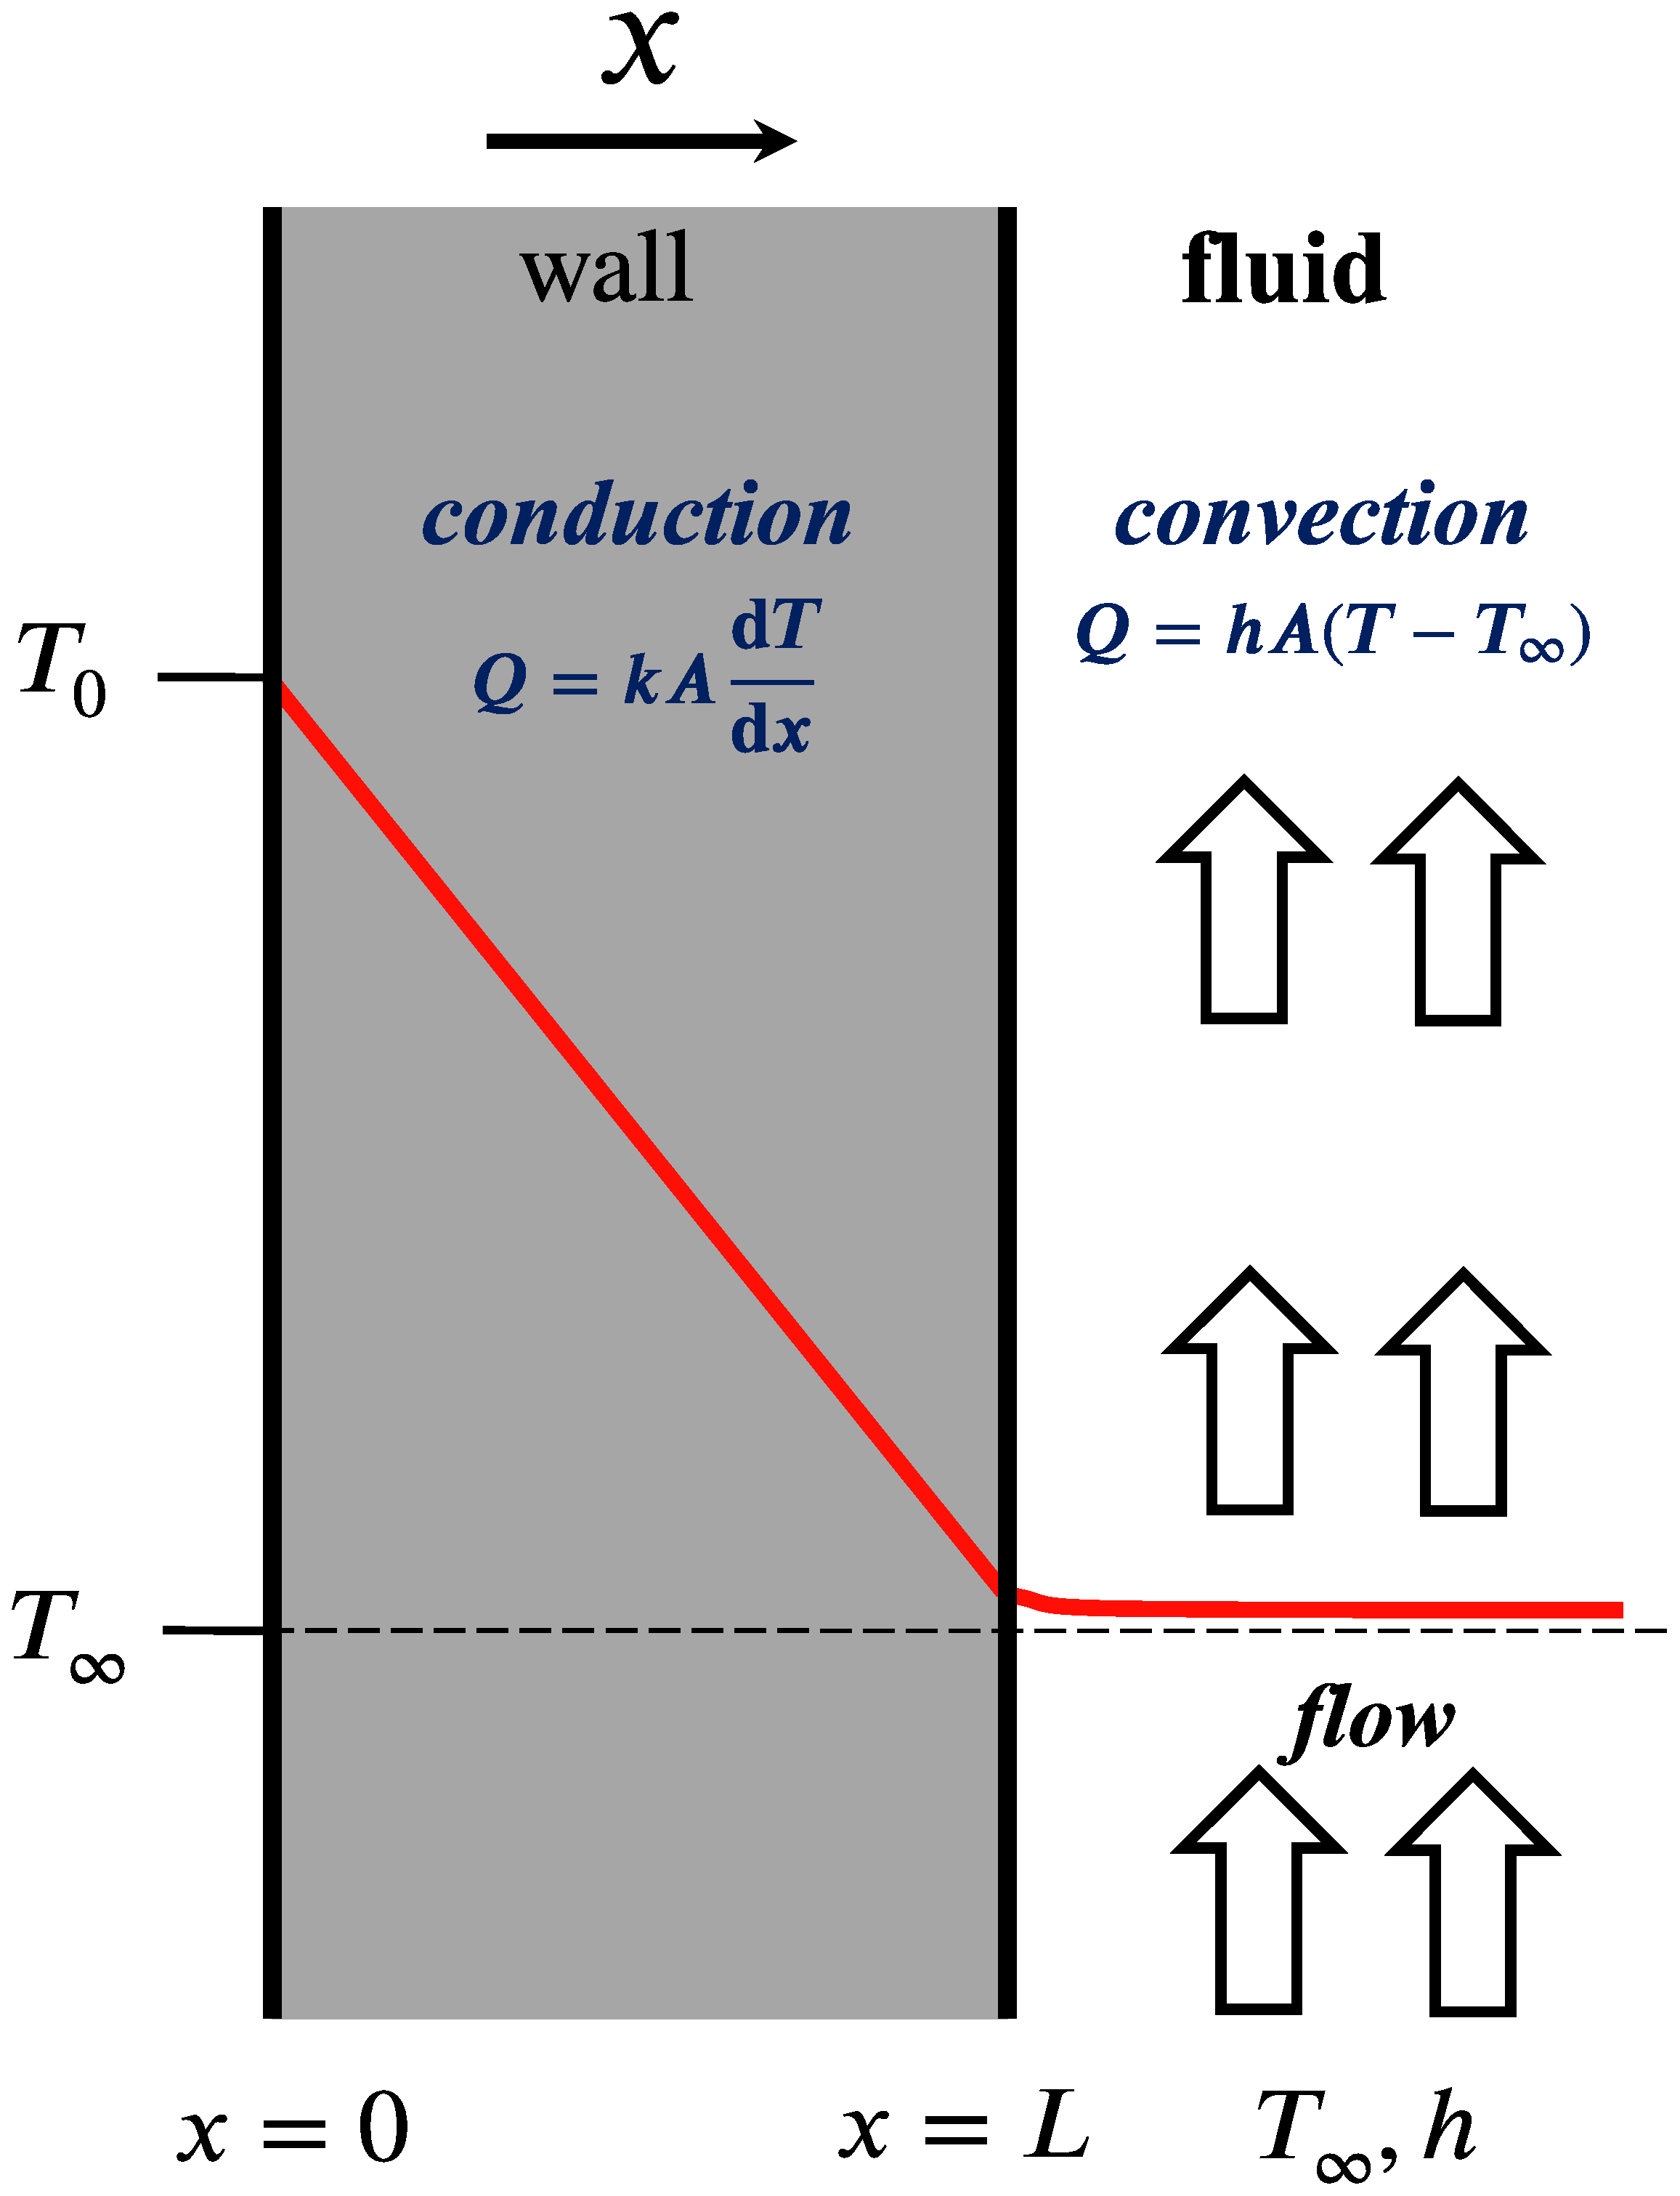
\includegraphics[width=\textwidth]{conduction-convection.eps}
    \end{figure}
\end{minipage}

\begin{itemize}
    \item Integral form of heat equation: 
    \[
        \underbrace{\frac{\partial}{\partial t} \int\limits_{CV} \rho c_{p} T \mathrm{d}V}_{\substack{\text{rate of change}\\\text{of thermal energy}}} = \underbrace{\int\limits_{CV} \dot{S_{v}} \mathrm{d}V}_{\substack{\text{rate of}\\ \text{heat generation}}} - \underbrace{\oint\limits_{CS} (\mathbf{q} \cdot \mathbf{n}) \mathrm{d}A}_{\substack{\text{rate of heat loss}\\\text{due to heat flux}}} - \underbrace{\oint\limits_{CS} \rho c_{p} T (\mathbf{v} \cdot \mathbf{n}) \mathrm{d}A}_{\substack{\text{rate of heat loss}\\ \text{by fluid flow across CS}}} 
    \]
    
    \item Differential form of heat equation: 
    \[ 
        \underbrace{\rho c_{p}\bigg(\frac{\partial T}{\partial t} +(\mathbf{v} \cdot \nabla)  T\bigg)}_{\text{rate of change of heat in fluid particle}} = \underbrace{\dot{S_{v}}}_{\substack{\text{rate of} \\ \text{heat generation}}}  + \underbrace{k \nabla^{2} T}_{\substack{\text{rate of heat} \\ \text{accumulation by conduction}}} 
    \]
\end{itemize}
%===========================================
\subsection{Steady-State Conduction}
\begin{minipage}{.7\textwidth}
\begin{table}[H]
    \centering
    \begin{tabular}{lc}
    \toprule
    & \textbf{Thermal Resistance, $R_{T}(\mathrm{K}/\mathrm{W})$}\\ 
    \midrule
    Conduction(planar)  & $L/kA$\\
    [1.3ex]
    Conduction(cylindrical) & $\displaystyle \frac{\ln(r_{2}/r_{1})}{2\pi Lk}$\\
    [1.6ex]
    Conduction(spherical)  & $\displaystyle \frac{1}{4\pi k}(\frac{1}{r_{1}}-\frac{1}{r_{2}})$\\ 
    [1.3ex]
    Convection &  \large{$1/hA$}\\
    \bottomrule
    \end{tabular}
\end{table} 
\end{minipage}
\begin{minipage}{.3\textwidth}
\begin{circuitikz} 
    \draw
        (0,0) node[label={[font=\footnotesize]above:$T_{1}$}]{} to [R, *-*, R=$R_T$, v=$\Delta T$] (3,0) node[label={[font=\footnotesize]above:$T_{2}$}]{};
\end{circuitikz}
\[
    \hspace{-2.5cm} \dot{Q} = \frac{\Delta T}{R_{T}} 
\]
\end{minipage}
%===========================================
\subsection{Transient Heat Conduction}
\begin{itemize}
    \item Lumped capacitance method: 
    \[
        T =(T_{i}-T_{\infty}) \ \exp(-\frac{t}{\tau})+T_{\infty} \quad \Rightarrow \ \frac{T-T_{\infty}}{T_{i}-T_{\infty}}=\exp(-\frac{t}{\tau}), \quad \tau=\frac{\rho c_{p} V}{hA}
    \] 
	
    \item Conduction through semi-infinite solid:
	\begin{itemize}
            \item Penetration depth of the “front”: $x  \sim  \sqrt{\alpha t}$
            
            \item Error function: $1-\mathrm{erf}(z)=\mathrm{erfc}(z)$
            \[
                T = (T_{s}-T_{i}) \ \mathrm{erfc}\bigg(\frac{x}{2\sqrt{\alpha t}}\bigg)+T_{i}
            \]
            
            \item Heat flux at the surface:
            \[
                q_{s} = \sqrt{\frac{k \rho c_{p}}{\pi t}}(T_{s}-T_{i})
            \]
            
            \item Interfacial temperature:
            \[
                T_{s}=\frac{T_{A}m_{A}+T_{B}m_{B}}{m_{A}+m_{B}}, \quad m_{A} = \sqrt{k_{A}\rho_{A}c_{p,A}}, \quad m_{B} = \sqrt{k_{B}\rho_{B}c_{p,B}}
            \]
	\end{itemize}
\end{itemize}
%===========================================
\subsection{Convective Heat Transfer}
\begin{itemize}
    \item Averaged convective coefficient: $\displaystyle \bar{h}=\frac{1}{A}\int h \ \mathrm{d}A_{S}$
    
    \item Thickness of the velocity boundary layer: $\delta_{v} \sim \sqrt{\nu t}$, where $\nu=\mu/\rho$
    
    \item Thickness of the thermal boundary layer: $\delta_{T} \sim \sqrt{\alpha t}$
    
    \item Given a thermal boundary layer, to find $h$:
    \[
        h=-\frac{k}{T_{s}-T_{\infty}}\frac{\mathrm{d}T}{\mathrm{d}y}\bigg\rvert_{y=0} 
    \]
    
    \item Reynolds Number 
    \[
        Re_{x} = \frac{\rho u_{\infty} x}{\mu}=\frac{u_{\infty}x}{\nu}
    \]

    \item Laminar flow over an isothermal \textit{flat plate}: $Re_{x}<<5\times 10^{5}$\\
    \begin{center}
    \begin{tabular}{lcc}
        $Pr<<1$ & $Nu_{x} = 0.564Re_{x}^{\frac{1}{2}}Pr^{\frac{1}{2}}$  & $\bar{Nu}_{L} =1.128Re_{L}^{\frac{1}{2}}Pr^{\frac{1}{2}}$\\ [1.3ex]  
        $Pr>0.5$ &  $Nu_{x} = 0.332Re_{x}^{\frac{1}{2}}Pr^{\frac{1}{3}}$ &   $\bar{Nu}_{L} =0.664Re_{L}^{\frac{1}{2}}Pr^{\frac{1}{3}}$ 
    \end{tabular}
    \end{center}
    
    \item Turbulent flow over an isothermal \textit{flat plate}: $5\times 10^{5}<Re_{x}<3\times 10^{7}$
    \begin{center}
    \begin{tabular}{l l}
        $0.7<Pr<400$ & $\displaystyle Nu_{x}=0.029Re_{x}^{0.8}Pr^{0.43}$\\
        & $\displaystyle \bar{Nu}_{L}=0.664Re_{c}^{\frac{1}{2}}Pr^{\frac{1}{3}}+0.036Re_{L}^{0.8}Pr^{0.43}\bigg[1-\bigg(\frac{Re_{c}}{Re_{L}}\bigg)^{0.8}\bigg]$
    \end{tabular}
    \end{center}

    \item Laminar, fully developed flow through a \textit{circular} pipe: $Re_{D}<<2300$
    \begin{center}
        \begin{tabular}{l l}
        Uniform surface heat flux (uniform $q_{h})$ & $Nu_{D}=4.36$ \\ [1.3ex]  
        Uniform surface temperature (uniform $T_{s}$) &  $Nu_{D}=3.66$	
    \end{tabular}
    \end{center}
    
    \item Turbulent flow, fully developed flow through a \textit{circular} pipe: $Re_{D}>10^{4}$, $Pr>0.7$
    \[Nu_{D} = 0.023 Re_{D}^{0.8}Pr^{0.4}\]

    \item Internal flow: 
    \begin{itemize}
        \item Hydrodynamic entrance length: $\displaystyle 
        x_{e,V} \approx 0.05 D \ Re_{D}$
        \item Thermal entrance length: $\displaystyle x_{e,T} \approx 0.05 D \ Re_{D} \ Pr$
        \item Mean temperature: $\displaystyle T_{m} = \frac{2\pi}{Q}\int_{0}^{R}T\ u\ r\ \mathrm{d}r$
    \end{itemize}
\end{itemize}
%===========================================
%===========================================
\section{Mass Transport}
\begin{minipage}{.6\textwidth}
\begin{table}[H]
    \centering
    \begin{tabular}{ccc}
    \toprule
    Advection   &   Diffusion   &   Convection \\
    \midrule
    $\mathbf{j}_{a}=C\mathbf{u}$    &   $\mathbf{j}_{d}=-\mathcal{D}\nabla C$ &   $\mathbf{j}_{k}=k_{m}(C-C_{m})$ \\
    \bottomrule
    \end{tabular}
\end{table}
\end{minipage}
\begin{minipage}{.3\textwidth}
\[
    \hspace{-2cm} \Rightarrow \quad \mathbf{j}_{\textrm{total}} = \mathbf{j}_{a} + \mathbf{j}_{d} = C\mathbf{u} - \mathcal{D}\nabla C
\]
\end{minipage}

\begin{itemize}
    \item Fick's First Law in 1-D
    \[j = -\mathcal{D}\frac{\partial C}{\partial x}\]
    
    \item Stokes-Einstein Equation 
    \[
    \mathcal{D}=\frac{k_{B}T}{6\pi \mu a}, \quad 
    a = \bigg(\frac{3M_w}{4\pi \rho N_A}\bigg)^{\frac{1}{3}}
    \]
    
    \item Integral form of conservation of solute of mass 
    \[
        \frac{\partial}{\partial t} \int\limits_{CV} C \mathrm{d}V = \int\limits_{CV} \dot{S_{v}} \mathrm{d}V - \oint\limits_{CS} (\mathbf{j} \cdot \mathbf{n}) \mathrm{d}A - \oint\limits_{CS} C (\mathbf{v} \cdot \mathbf{n}) \mathrm{d}A 
    \]
    
    \item Differential form of conservation of solute of mass
    \[
        \frac{\partial C}{\partial t} + (\mathbf{v} \cdot \nabla)C = \mathcal{D}\nabla^2 C + \dot{S}_{v}
    \]
\end{itemize}
%===========================================
%===========================================
\vspace*{\fill}
\framebox{\href{https://www.overleaf.com/read/gqtthbzjbfpd}{Scripted} by B Li \& P Xie. \ Last update: \today}


\end{document}